\documentclass[a4paper,10pt]{article}
\usepackage[margin=0.48in]{geometry}
\usepackage{graphicx}
\usepackage{array}
\usepackage{ragged2e}
\usepackage[none]{hyphenat}

\renewcommand{\baselinestretch}{1.12}
\setlength{\parindent}{0pt}
\pagestyle{empty}
\enlargethispage{2\baselineskip}

\begin{document}
\centering

\begin{tabular}{|l@{\hspace{1.5em}}|>{\raggedright\arraybackslash}p{13.6cm}|}
\hline

% --- 1. TITLE ---
\multicolumn{2}{|p{18cm}|}{
  \centering \vspace{0.18cm}
  \textbf{\large Nutriloop: A Deep Learning and Generative AI-Driven Diet Recommendation System for Personalized Chronic Disease Management}\par
  \vspace{0.18cm}
} \\
\hline

% --- 2. DOMAIN ---
\multicolumn{2}{|p{18cm}|}{
  \vspace{0.12cm}
  \textbf{Domain:} Clinical Decision Support Systems, Machine Learning \& Deep Learning, Generative AI / Large Language Models, Healthcare \& Preventive Nutrition\par
  \vspace{0.12cm}
} \\
\hline

% --- 3. ABSTRACT ---
\multicolumn{2}{|p{18cm}|}{
  \vspace{0.12cm}
  \textbf{Abstract:}\par\vspace{0.12cm}
  \justifying
  Chronic kidney disease (CKD), hypertension (HTN) and type 2 diabetes (T2DM) often occur together, and the diets written for each can contradict one another: DASH raises potassium, which a failing kidney cannot clear. Nutriloop is an offline clinical decision support system that turns a lab report into a seven-day meal plan. HistGradientBoosting models with Platt calibration, trained on 1,224,788 records from five public sources, estimate the risk of each disease.\par\vspace{0.16cm}
  
  A deterministic engine converts risk into KDIGO, ADA and DASH limits, resolves conflicts renal-first, screens 31 medication keys and 11 allergen classes, and plans meals in five regional cuisines. An LLM agent can change a plan only through the same checks. Held-out ROC-AUC was 0.921, 0.954 and 0.928, and an audit of 500 plans found no violations. The system runs as a standalone Windows application.\par\vspace{0.20cm}

  \textbf{Keywords:} clinical decision support, chronic kidney disease, hypertension, type 2 diabetes, comorbidity, diet recommendation, probability calibration, large language models.\par
  \vspace{0.12cm}
} \\
\hline

% --- 4. ARCHITECTURE / FLOW DIAGRAM ---
\multicolumn{2}{|p{18cm}|}{
  \vspace{0.12cm}
  \textbf{Architecture / Flow Diagram:}\par\vspace{0.15cm}
  \begin{center}
    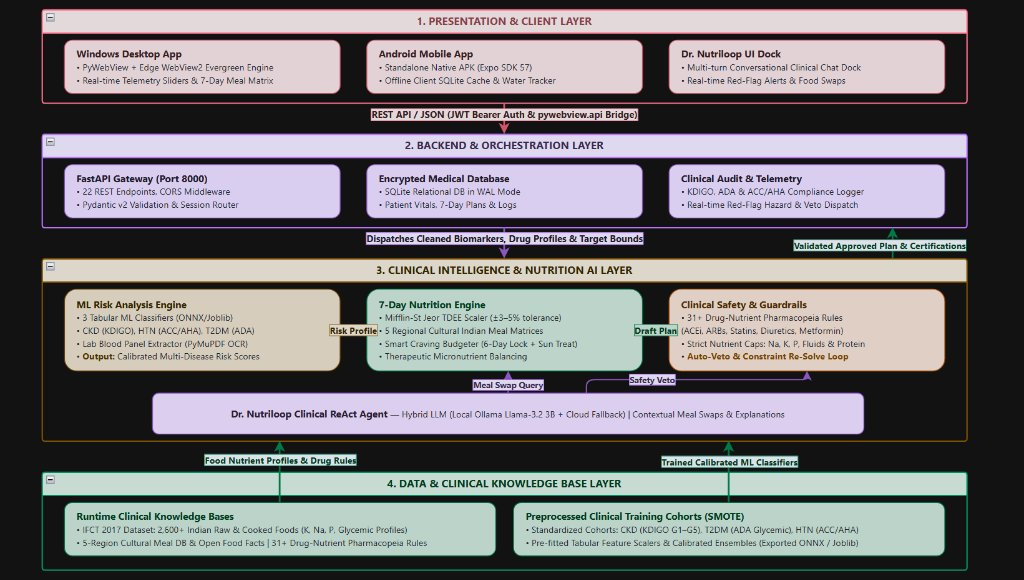
\includegraphics[width=17.2cm, height=9.6cm, keepaspectratio]{architecture.png}
  \end{center}
  \vspace{0.08cm}
} \\
\hline

% --- 5. SUPERVISOR & TEAM ---
\begin{tabular}[t]{@{}l@{}}
  \textbf{Supervisor:} \\[0.8ex]
  Dr. Saritha K. \\[0.2ex]
  \small Associate Professor
\end{tabular}
&
\begin{tabular}[t]{@{}l@{}}
  \textbf{Team No.:} 17 \\[0.8ex]
  \begin{tabular}[t]{@{}l@{\hspace{1.1cm}}l@{\hspace{1.1cm}}l@{\hspace{1.1cm}}l@{}}
    \small\textbf{Vatsal Jain} & \small\textbf{Vivek Tutika} & \small\textbf{Pranav Shetty} & \small\textbf{Sourabh S. Hegde} \\[0.3ex]
    \small PES2UG23CS681 & \small PES2UG23CS707 & \small PES2UG23CS721 & \small PES2UG23CS929
  \end{tabular}
\end{tabular} \\
\hline

% --- 6. PUBLICATION ---
\multicolumn{2}{|p{18cm}|}{
  \vspace{0.001cm}
  \textbf{Publication:}\par\vspace{0.25cm}
  \textbf{Status:}\par
  \vspace{3cm}
  \textbf{ }\par
} \\
\hline

\end{tabular}

\end{document}
